\documentclass{../paper}

\newcommand{\todo}[1]{\textcolor{red}{To-do: #1}}

\begin{document}

\title{Measurement of the Muon Lifetime and the Fermi Coupling Constant}

\author{Iago B.~Mendes\,\orcidlink{0009-0007-9845-8448}}
\email{ibrazmen@oberlin.edu}
\affiliation{Department of Physics and Astronomy, Oberlin College, Oberlin, Ohio 44074, USA}

\date{\today}

\begin{abstract}
  Muons, produced by cosmic rays in the upper atmosphere, experience relativistic time dilation, which extends their lifetime and allows them to reach Earth's surface. In this experiment, we measured their lifetime by observing their decay in a plastic scintillator detector. By recording the muon decay times and fitting the data to an exponential decay model, we determined a charge-averaged lifetime of $\tau = 2.10(2) \ \mu s$, which lies within the literature values for the lifetime of positive and negative muons. From the measured lifetime, we estimated the reduced Fermi coupling constant, obtaining a value of $\bar G_F = 1.190(6) \times 10^{-5} \, \text{GeV}^{-2}$, which shows some expected disagreement with the literature value due to the charge-averaging nature of the experiment. These results provide valuable insights into how precise measurements advance our understanding of particle physics.
\end{abstract}

\maketitle

\section{Introduction}

Muons were first discovered in 1936 by Carl D. Anderson and Seth Neddermeyer while studying cosmic radiation \cite{Anderson1936}. They observed particles that curved differently from electrons and protons in a magnetic field, suggesting an intermediate mass. The existence of these particles was confirmed in the following year \cite{Street1937}.

The role of muons in the study of the weak interaction was gradually established in the years after their discovery. Initially, muons were thought to be part of the meson family, which had been hypothesized by Yukawa to mediate the strong nuclear force \cite{Yukawa1935}. However, the work of Conversi, Piccioni, and Pancini revealed that muons decay in a manner inconsistent with strong interaction mediators \cite{Conversi1946}. Instead, it was found that muons decay via the weak interaction, like electrons, but with a longer lifetime. This led to the realization that muons were leptons and that their behavior was governed by the weak nuclear force. The theoretical framework for weak interactions had been proposed earlier by Enrico Fermi in 1933 in the context of beta decay, introducing the Fermi coupling constant $G_F$ \cite{Fermi1933}.

In the modern era, muon lifetime measurements such as the one reported here remain important for testing the foundations of the Standard Model. Precise measurements of the muon lifetime allow for increasingly accurate determinations of $G_F$ \cite{Chitwood2007}. By reproducing one of the key results in particle physics history, the experiment in this report provides an accessible way to explore the weak force and extract a fundamental physical constant from direct observation.

In this experiment, we used a plastic scintillator detector to measure the lifetime of muons. With this measurement, we estimated the Fermi coupling constant. In Section~\ref{sec:theory}, we provide an overview of muon decay and its connection to the Fermi coupling constant. Section~\ref{sec:methods} describes the working principles of the scintillator detector and our experimental procedures. Section~\ref{sec:results} presents our results and analysis. Finally, we conclude in Section~\ref{sec:conclusion} with a summary of our findings and possible areas of improvement.

\section{Theory} \label{sec:theory}

Cosmic rays are high-energy particles originating from space, primarily composed of protons. When these cosmic rays strike nuclei in the upper atmosphere, they produce secondary particles. Among these, we find charged pions, which decay into muons through
\begin{equation}
  \pi^+ \to \mu^+ + \nu_\mu
\end{equation}
and
\begin{equation}
  \pi^- \to \mu^- + \bar\nu_\mu.
\end{equation}
These muons then continue traveling toward Earth's surface.

Given that muons have a lifetime on the order of $\sim 1 \ \mu s$ and it takes about $\sim 1 \ ms$ to travel from the upper atmosphere to sea level at relativistic speeds, one might question how we are able to detect muons in Earth's surface. The answer relies on time dilation \cite{TeachSpinManual}, which extends their lifetime from our point of view as stationary observers on Earth.

Once slowed down in our detector, muons decay into electrons or positrons via
\begin{equation}\label{eq:muon-decay}
  \mu^- \to e^- + \bar\nu_e + \nu_\mu
\end{equation}
or
\begin{equation}\label{eq:muon+decay}
  \mu^+ \to e^+ + \nu_e + \bar\nu_\mu,
\end{equation}
respectively. Our goal in this experiment is to build a distribution of the decay times of Eqs.~\eqref{eq:muon-decay}--\eqref{eq:muon+decay} inside the detector.

If we were to account for the time it takes for muons to travel from the upper atmosphere to our detector, we would get a distribution that follows an exponential decay of the form
\begin{equation}\label{eq:exponential-decay}
  N(t) = N_0 e^{-t/\tau}
\end{equation}
\cite{TeachSpinManual}, where $N(t)$ is the number of muons decaying after time $t$, $N_0$ is the starting number of muons, and $\tau$ is the muon lifetime. Fortunately, if we instead account only for the time that muons stay in our detector, we obtain the same exponential form $e^{-t/\tau}$, which is independent of $N_0$. Therefore, by fitting our histogram of measured decay times to a function like Eq.~\eqref{eq:exponential-decay}, we can extract an experimental value for $\tau$.

The muon decays in Eqs.~\eqref{eq:muon-decay}--\eqref{eq:muon+decay} occur via the weak interaction. The strength of this weak force is given by the Fermi coupling constant $G_F$, which is related to the particle's lifetime $\tau$ by
\begin{align}\label{eq:Fermi-constant}
  G_F = \sqrt{192 \pi^3 \frac{\hbar^7}{\tau m^5 c^4}}
\end{align}
\cite{TeachSpinManual}, where $m$ is the particle's mass. Hence, by measuring the muon lifetime, we can estimate $G_F$.

\section{Methods} \label{sec:methods}

\begin{figure}
  \centering
  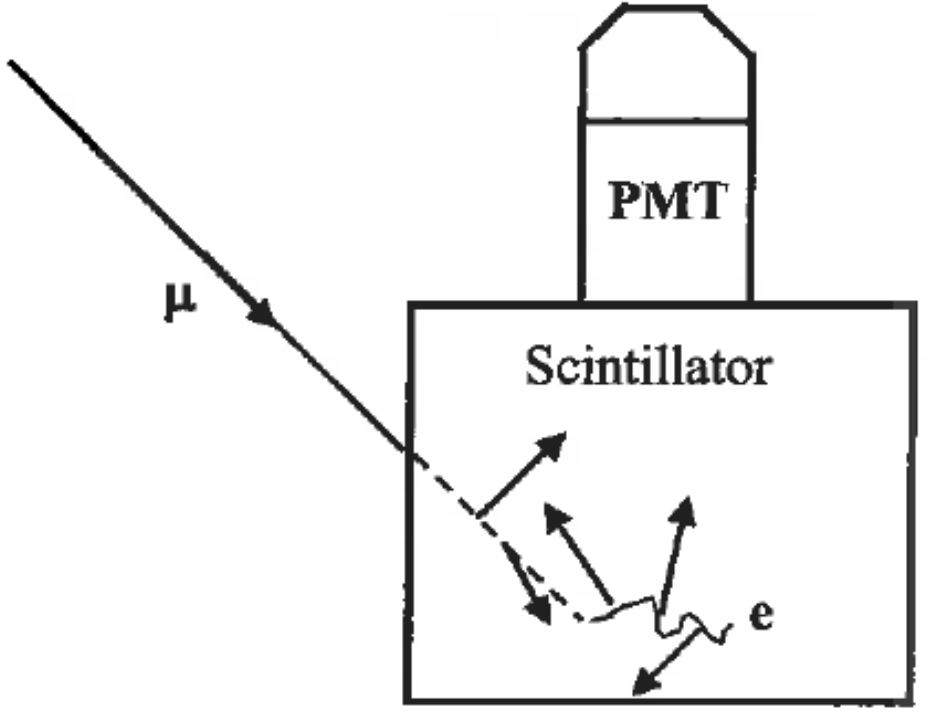
\includegraphics[width=0.6\columnwidth]{assets/detector.png}
  \caption{Schematic showing the two pulses created in the scintillator and detected by a photomultipler tube (PMT). This figure is reproduced from \cite{TeachSpinManual}.}
  \label{fig:detector}
\end{figure}

To measure the lifetime of the muon, we use a plastic scintillator detector (FIG.~\ref{fig:detector}), which works by identifying muons that stop inside the scintillator and subsequently decay. When a muon enters the scintillator, it slows down and eventually stops, ionizing the scintillator material in the process. This ionization produces a pulse of scintillation light, which is detected and starts a timing clock \cite{TeachSpinManual}.

After coming to rest, the muon decays according to Eq.~\eqref{eq:muon-decay} or Eq.~\eqref{eq:muon+decay}. The resulting electron or positron emerges with significant kinetic energy and ionizes the scintillator material as it passes through, producing a second pulse of light and stopping the clock \cite{TeachSpinManual}. The time interval between the two pulses then corresponds to the muon's lifetime inside the detector.

The detector's ability to accurately and precisely measure decay times is limited by two main factors. First, its time resolution affects how well we can distinguish short lifetimes. This becomes important when fitting our data to an exponential decay model, as discussed in the next section. Second, extraneous single-event signals affect the start and stop triggers of our timing clock. These could be background signals -- caused by cosmic rays or environmental radiation -- or muons that do not decay inside the detector and instead pass through it.

To address such single-event effects, the detector includes an interval limit. Once the first scintillation pulse is recorded, the system waits up to 20,000 $ns$ for a second pulse \cite{TeachSpinManual}. If no second pulse is detected in that period, the event is discarded. This helps ensure that only valid decay events are included in our data.

One might worry that overlapping muon decays will break our timing clock strategy, but this is not a concern given how often we have muon decays in our detector. Over the course of 20 seconds, we can estimate that 97 single events occur based on \cite{Sage}. That is, we have a rate of $\sim 5$ single events per second. Over the course of 599,405 seconds, we recorded 12,608 muon decays. That is, we have a rate of $\sim 0.02$ muon decay per second. Therefore, at each second, the probability of a muon stopping is $\sim 0.4\%$. This means that it is very unlikely for more than one muon to decay at the same time, allowing us to treat each decay as an independent event.

\section{Results} \label{sec:results}

\begin{figure*}
  \centering
  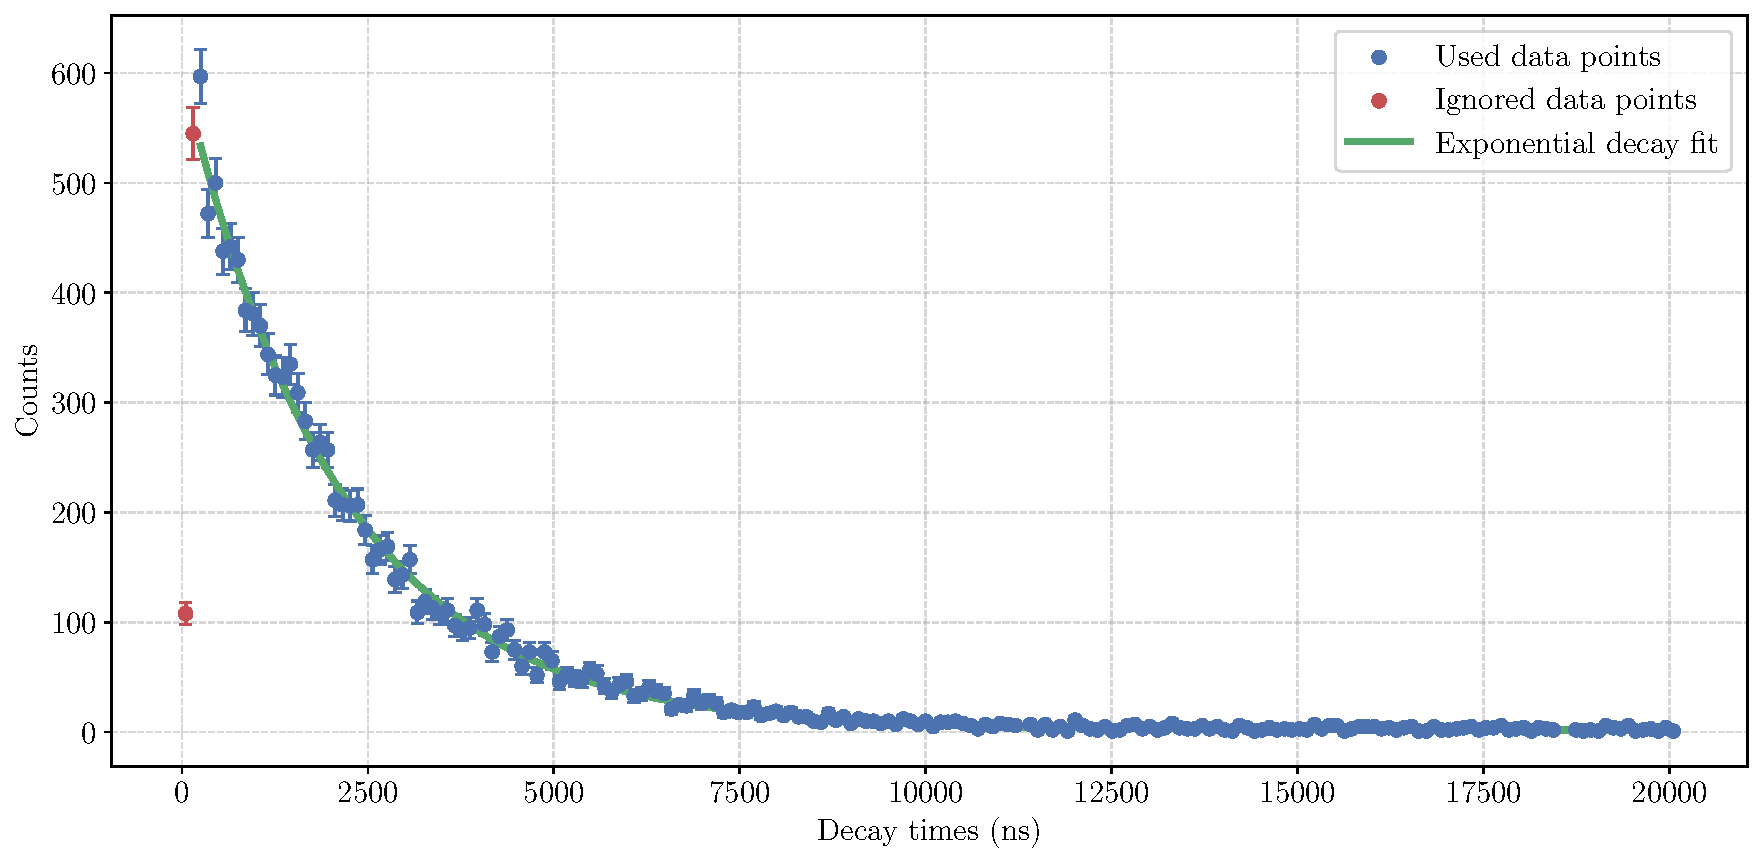
\includegraphics[width=\textwidth]{data/analysis.pdf}
  \caption{Histogram of muon decay times.}
  \label{fig:analysis}
\end{figure*}

A histogram of our measured decay intervals is shown in FIG.~\ref{fig:analysis}. To find the best possible binning strategy of our data, we perform the following steps for each given number of bins $N$.
\begin{enumerate}
  \item Calculate bin width.
  \item Categorize data into bins.
  \item Remove any empty bins.
  \item Find bin with the maximum count and ignore any bins before it.
  \item Calculate the uncertainty of each bin $i$ with $N_i$ counts as $\delta N_i = \sqrt{N_i}$.
  \item Use {\tt SciPy}'s {\tt curve\_fit} procedure \cite{SciPy} to fit our data as an exponential decay of the form
    \begin{equation}
      N(t) = A e^{-t/\tau} + C,
    \end{equation}
    where $A$ is the amplitude, $\tau$ is the timescale, and $C$ is a vertical offset.
  \item Calculate reduced chi squared $\bar\chi^2$.
\end{enumerate}

Note that step 4 is needed in order to address the time resolution limitation of the detector. By starting the fit at the bin with the maximum count, we ignore bins at under-resolved times.

We performed steps 1--7 for all $50 \leq N \leq 500$ (at incremental steps of 5). We found the best reduced chi squared value,
\begin{equation}
  \bar\chi^2 = 1.007,
\end{equation}
with $N=200$ bins (out of which 195 bins remain after steps 3 and 4). With this, our measurement for the lifetime of the muon is
\begin{equation}\label{eq:muon-decay-value}
  \tau = 2.10(2) \ \mu\text{s},
\end{equation}
where the uncertainty $\delta\tau$ was taken directly from the fit standard deviation.

As mentioned in the previous section, both positive and negative muons interact with the atoms in the scintillator material, producing scintillation light upon entry. However, negative muons can also be captured by the protons in the nuclei, leading to an alternate decay pathway given by 
\begin{equation}
  \mu^- + p \to n + \nu_\mu
\end{equation}
\cite{TeachSpinManual}. Because of this, $\mu^-$ has a lower lifetime compared to $\mu^+$ \cite{TeachSpinManual}. Hence, Eq.~\eqref{eq:muon-decay-value} is a charge-averaged measurement of the lifetime of the muon.

From \cite{TeachSpinManual}, we know that the literature lifetimes of $\mu^+$ and $\mu^-$ are
\begin{equation}\label{eq:tau+}
  \tau^+ = 2.19703(2) \ \mu s
\end{equation}
and
\begin{equation}\label{eq:tau-}
  \tau^- = 2.043(3) \ \mu s,
\end{equation}
respectively. Based on \cite{TeachSpinManual}, we know that we can find the ratio of the number of $\mu^+$ and the number of $\mu^-$ as
\begin{align}
  \rho
  &= -\frac{\tau^+}{\tau^-} \left(\frac{\tau^- - \tau}{\tau^+ - \tau}\right) \\
  &= 0.6(4). \label{eq:ratio}
\end{align}

Note that the error in Eq.~\eqref{eq:ratio} is very large. It was computed using the error propagation formula
\begin{equation}\label{eq:rho-error}
  \delta\rho = \frac{\tau^+}{\tau^-} \frac{(\tau^+ - \tau^-)}{(\tau^+ - \tau)^2} \delta\tau,
\end{equation}
where we are ignoring the uncertainties $\delta\tau^+$ and $\delta\tau^-$ in Eqs.~\eqref{eq:tau+}--\eqref{eq:tau-} because the uncertainty $\delta\tau$ in Eq.~\eqref{eq:muon-decay-value} dominates. Eq.~\eqref{eq:rho-error} can be recast as
\begin{equation}\label{eq:rho-relative-error}
  \frac{\delta\rho}{\rho} = \frac{\tau (\tau^+ - \tau^-)}{(\tau^+ - \tau) (\tau - \tau^-)} \frac{\delta\tau}{\tau}.
\end{equation}
Using our experimental values, Eq.~\eqref{eq:rho-relative-error} becomes
\begin{equation}\label{eq:rho-relative-error-numeric}
  \frac{\delta\rho}{\rho} = 58.5\ \frac{\delta\tau}{\tau}.
\end{equation}
This tells us that the error in $\tau$ significantly amplifies the error in $\rho$. Then, to get a more accurate value of $\rho$, we need a much more accurate measurement of $\tau$.

Let's now determine the Fermi coupling constant, which is related to the muon lifetime by Eq.~\eqref{eq:Fermi-constant}. In natural units, we define the reduced Fermi constant as
\begin{equation}
  \bar G_F = \frac{G_F}{(\hbar c)^3} = \sqrt{ 192 \pi^3 \frac{\hbar}{\tau (m c^2)^5} }.
\end{equation}
Using $\hbar = 6.5821 \times 10^{-16} \ eV \cdot s$ \cite{NIST_hbar} and $m c^2 = 105.66 \ MeV$ \cite{NIST_muon}, we find
\begin{equation}\label{eq:Fermi-constant-value}
  \bar G_F = 1.190(6) \times 10^{-5} \ GeV^{-2},
\end{equation}
where the uncertainty was calculated with
\begin{equation}
  \frac{\delta \bar G_F}{\bar G_F} = \frac{1}{2} \frac{\delta \tau}{\tau}.
\end{equation}
Compared to the literature value, $1.1663 \times 10{-5} \ GeV^{-2}$ \cite{NIST_Fermi}, our measurement in Eq.~\eqref{eq:Fermi-constant-value} is significantly larger. This is expected since we found that our $\tau$ is smaller than the literature value of $\mu^+$ due to the extra interaction of $\mu^-$ with matter.

\section{Conclusion} \label{sec:conclusion}

Using a plastic scintillator detector, we measured the charge-averaged muon lifetime and obtained a value of $\tau = 2.10(2) \ \mu s$, which is in reasonable agreement with literature values for positive and negative muons. From this, we determined the ratio of positive to negative muons to be $\rho = 0.6(4)$. Finally, we estimated the reduced Fermi coupling constant as $\bar G_F = 1.190(6) \times 10^{-5} \, \text{GeV}^{-2}$, which -- as expected -- is larger than the accepted value due to the charge-averaging nature of our measurement. These results provide a direct observation of the weak interaction through muon decay, making the experiment not only a valuable exercise in particle detection techniques, but also a meaningful link to the historical development of particle physics.

Despite the success of the experiment, the large uncertainty in $\rho$ highlights the need for improved accuracy. Future experiments could benefit from increased time resolution, longer data collection periods to build a larger sample size, and better suppression of background noise. An additional improvement would be to separate positive and negative muons in our detector, allowing us to measure their individual lifetimes. This would enable the estimation of the true Fermi coupling constant using only positive muons.

\begin{acknowledgements}
  This work was done in collaboration with Avay Subedi and John Duffy under the supervision of Professor Yumi Ijiri.
\end{acknowledgements}

\bibliography{refs}

\end{document}
